%%
%% Copyright 2007, 2008, 2009 Elsevier Ltd
%%
%% This file is part of the 'Elsarticle Bundle'.
%% ---------------------------------------------
%%
%% It may be distributed under the conditions of the LaTeX Project Public
%% License, either version 1.2 of this license or (at your option) any
%% later version.  The latest version of this license is in
%%    http://www.latex-project.org/lppl.txt
%% and version 1.2 or later is part of all distributions of LaTeX
%% version 1999/12/01 or later.
%%
%% The list of all files belonging to the 'Elsarticle Bundle' is
%% given in the file `manifest.txt'.
%%

%% Template article for Elsevier's document class `elsarticle'
%% with numbered style bibliographic references
%% SP 2008/03/01
%%
%%
%%
%% $Id: elsarticle-template-num.tex 4 2009-10-24 08:22:58Z rishi $
%%
%%
\documentclass[preprint,12pt,3p]{elsarticle}

%% Use the option review to obtain double line spacing
%% \documentclass[preprint,review,12pt]{elsarticle}

%% Use the options 1p,twocolumn; 3p; 3p,twocolumn; 5p; or 5p,twocolumn
%% for a journal layout:
%% \documentclass[final,1p,times]{elsarticle}
%% \documentclass[final,1p,times,twocolumn]{elsarticle}
%% \documentclass[final,3p,times]{elsarticle}
%% \documentclass[final,3p,times,twocolumn]{elsarticle}
%% \documentclass[final,5p,times]{elsarticle}
%% \documentclass[final,5p,times,twocolumn]{elsarticle}

%% if you use PostScript figures in your article
%% use the graphics package for simple commands
%% \usepackage{graphics}
%% or use the graphicx package for more complicated commands
%% \usepackage{graphicx}
%% or use the epsfig package if you prefer to use the old commands
%% \usepackage{epsfig}

%% The amssymb package provides various useful mathematical symbols
\usepackage{amssymb}
%% The amsthm package provides extended theorem environments
%% \usepackage{amsthm}

%% The lineno packages adds line numbers. Start line numbering with
%% \begin{linenumbers}, end it with \end{linenumbers}. Or switch it on
%% for the whole article with \linenumbers after \end{frontmatter}.
\usepackage{lineno}
\usepackage{booktabs}
\usepackage{longtable}
\usepackage{tabu}
\usepackage{xcolor}
\usepackage{float}
\usepackage{hyperref}
\usepackage{todonotes}
\newcommand{\noteZN}[1]{\footnote{\textcolor{red}{#1}}}

%% natbib.sty is loaded by default. However, natbib options can be
%% provided with \biboptions{...} command. Following options are
%% valid:

%%   round  -  round parentheses are used (default)
%%   square -  square brackets are used   [option]
%%   curly  -  curly braces are used      {option}
%%   angle  -  angle brackets are used    <option>
%%   semicolon  -  multiple citations separated by semi-colon
%%   colon  - same as semicolon, an earlier confusion
%%   comma  -  separated by comma
%%   numbers-  selects numerical citations
%%   super  -  numerical citations as superscripts
%%   sort   -  sorts multiple citations according to order in ref. list
%%   sort&compress   -  like sort, but also compresses numerical citations
%%   compress - compresses without sorting
%%
%% \biboptions{comma,round}

% \biboptions{}


\journal{Renewable \& Sustainable Energy Reviews}

\begin{document}

\begin{frontmatter}

\title{A review of unsupervised statistical learning and visual analytics techniques applied to  performance analysis of non-residential buildings}

% \texttt{elsarticle} class\tnoteref{label0}}
% \tnotetext[label0]{This is only an example}

\author{Clayton Miller}
\ead{miller.clayton@arch.ethz.ch}
\ead[url]{http://systems.arch.ethz.ch/}

\author{Zolt\'an Nagy}
\author{Arno Schlueter}

\address{ETH Z\"urich, Institute of Technology in Architecture (ITA), Architecture and Building Systems (A/S)}
\address{John-von-Neumann-Weg 9, Z\"urich, Switzerland} %\fnref{label4} [label2]



% \author{Author Two}
% \address{Some University}
% \ead{author.two@mail.com}

% \author{Author Three}
% \ead{author.three@mail.com}

\begin{abstract}
Measured and simulated data sources from the built environment are increasing rapidly. It is becoming normal to analyze data from hundreds, or even thousands of buildings at once. Mechanistic, manual analysis of such data sets is time-consuming and not realistic using conventional techniques. Thus, a significant body of literature has been generated using unsupervised statistical learning techniques designed to uncover structure and information quickly with fewer input parameters or meta data about the buildings collected. Further, visual analytics techniques are developed as aids in this process for a human analyst to utilize and interpret the results. This paper reviews publications that include the use of unsupervised machine learning techniques as applied to non-residential building performance control and analysis. The categories of techniques covered include clustering, novelty detection, motif and discord detection, rule extraction, and visual analytics. The publications apply these technologies in the domains of smart meters, portfolio analysis, operations and controls optimization, and anomaly detection. A discussion is included of key challenges resulting from this review, such as the need for better collaboration between several, disparate research communities and the lack of open, benchmarking data sets. Opportunities for improvement are presented including methods of reproducible research and suggestions for cross-disciplinary cooperation.

\end{abstract}

\begin{keyword}
building performance analysis \sep data mining \sep unsupervised learning \sep visual analytics \sep clustering \sep novelty detection \sep smart meter analysis \sep portfolio analysis \sep review \sep building controls and optimization
\end{keyword}

\end{frontmatter}

%%
%% Start line numbering here if you want
%%
% \linenumbers


%% main text
\section{Introduction}
\label{Introduction}
The creation and consolidation of measured sensor sources from the built environment and its occupants is occurring on an unprecedented scale. The Green Button Ecosystem now enables the easy extraction of data from over 60 million buildings\footnote{According to: http://www.greenbuttondata.org/}. Advanced metering infrastructure (AMI), or smart meters, have been installed on over 58.5 million buildings in the US alone \cite{energy_information_administration_how_2015}. The Internet-of-Things (IoT) movement provides an array of low-cost sensors, data acquisition devices, and cloud storage. A recent study has predicted a \$70-150 billion impact of IoT in offices and \$200-350 billion in homes \cite{james_manyika_unlocking_2015}. A recent press release from the White House summarizes the impact of utilities and cities in unlocking these data \cite{the_white_house_fact_2016}. It announces that 18 utilities, serving more than 2.6 million customers, will provide detailed energy data by 2017. This study also suggests that such accessibility will enable improvement of energy performance in buildings by 20\% by 2020. A vast majority of these raw data being generated are sub-hourly temporal data from meters and sensors. 

Ruparathna et al. created a contemporary review of building performance analysis techniques for commercial and institutional buildings \cite{ruparathna_improving_2016}. This review was comprehensive in capturing approaches related to technical, organizational, and behavioral changes. The majority of publications considered fall within the domains of automated fault detection and diagnostics, retrofit analysis, building benchmarking, and energy auditing. These traditional techniques focus on one building or a small, related collection of buildings, such as a campus. Many require complex characteristic data about each building, such as it geometric dimensions, building materials, the age of type of mechanical systems, and other metadata, to execute the process. 

Thus, a critical issue facing the building industry is how these traditional performance analysis techniques can utilize the current explosion of detailed, temporal sources. \emph{If one has access to raw data from thousands, or even millions, of buildings, how can analysis be scaled in a reasonable way?} Someone tasked with this type of analysis needs to extract information with less known meta-data about each building and fewer inputs into the process. In response to this question, researchers from several domains have developed methods of extracting insight from raw, unlabeled data from the built environment. Often these methods fall into the category of unsupervised statistical learning. Methods from this sub-domain of machine learning are advantageous due to their ability to characterize measured or simulated performance data quickly with less analyst intervention, metadata, and ground truth labeled data. They are often used in conjunction with visual analytics approaches as the first pass in the analysis of a large dataset.

A major challenge in utilizing this body of knowledge is that unsupervised machine learning techniques have been proposed, tested, and applied concurrently in several research domains and sub-domains. This situation has resulted in parallel, and mostly non-overlapping, collections of work with similar objectives, yet different publication venues and terminology. This review seeks to quantify this situation through an overview of the use of unsupervised learning techniques developed for the building industry. This task is done more holistically than previous reviews by combining key publications from a larger set of category applications and research domains. This overview is the first to specifically target unsupervised learning and visual analytics techniques for this context. The research sectors of building energy analysis, building simulation, computer science and electrical engineering are analyzed. This paper compiles a set of 100 publications released since 2005 that focus on the use of unsupervised statistical learning techniques on temporal or spatial data from non-residential buildings.

The paper is structured as follows, Section \ref{Techniques} gives background on the unsupervised machine learning used in the publications. Section \ref{Overview} provides an overview of various trends and statistics about the publications, including specific methods, the yearly timeline of release, and which research domains and specific journal and conference publications contain them. Sections \ref{SmartMeter}-\ref{AnomalyDetection} evaluate each of the publication categories in-depth. Finally, Section \ref{discussion} provides a discussion of the challenges observed and potential opportunities discovered through the review process. 


\subsection{Previous Reviews}
Various reviews have been completed that overlap with a part of the scope of this paper. Most of them are designed to focus on a single core domain of research; the main two areas are building operations analysis and smart grid optimization. One of the earliest reviews of artificial intelligence techniques for buildings was completed in 2003 by Krarti and covered both supervised and unsupervised methods \cite{krarti_overview_2003}. Dounis updated this work and focused on outlining specific techniques in detail \cite{dounis_artificial_2010}.  Reddy's seminal book about a large variety of analysis techniques for energy engineers includes chapters on clustering and unsupervised methods specifically \cite{reddy_applied_2011}. Lee et al. describe a variety of retrofit analysis toolkits which incorporate unsupervised and visual analytics approaches in a practical sense \cite{lee_energy_2015}. Ioannidis et al. created a large ontology of data mining and visual analytics for building performance analysis, however with a strong focus on the techniques and not examples of works using them \cite{ioannidis_big_2015}. From the utility and power grid side, Morias et al. created a general overview of various data mining techniques as focused on power distribution systems \cite{morais_overview_2009}. Chicco covered clustering methods specifically focused on load profiling tasks \cite{chicco_overview_2012}. Zhou et al. included the concept of customer load classification  \cite{zhou_review_2013}.\\


\section{Background of Unsupervised Learning and Visual Analytics Techniques}
\label{Techniques}
This section gives an overview of the five categories of unsupervised learning and visual analytics techniques discussed in this paper: clustering, novelty detection, motif and discord detection, rule extraction, and visual analytics. The general nature of the techniques is discussed, and the specific methods are briefly listed along with the abbreviations that are used in Tables \ref{fig:smart_table}-\ref{fig:anom_table}.

Statistical learning can be divided into two major categories: supervised learning and unsupervised learning. According to the formative text on the subject by James et al. and Hastie et al., supervised statistical learning techniques involve a set of observations $x_i, i = 1,....,n$ and an associated response variable $y_i$ \cite{james_introduction_2013,hastie_elements_2009}. The goal of a supervised process is to predict $y_i$ using the features generated from $x_i$; this objective is straightforward to verify according to the algorithms accuracy in predicting that response. Unsupervised learning, in contrast, lacks the associated response $y_i$ because it seeks merely to understand the relationship between the observations in $x_i$, generally in an exploratory fashion. These references go on to explain that unsupervised techniques are, thus, often more subjective in their application and are considered more challenging in their utilization in practical applications \cite{mirkin_clustering:_2012,james_introduction_2013,hastie_elements_2009}. Despite the challenge, various instances of their implementation are found in the literature with relation to building performance data as outlined in the subsequent sub-sections.\\

\subsection{Clustering}
Clustering is the most common general unsupervised approach applied to building performance data. It is used automatically to generate \emph{subgroups} of similar types of observations. James et al. describe this process as the grouping of $n$ observations into $K$ groups, or clusters, according to a set of generated $p$ features \cite{james_introduction_2013}. The two most common types of clustering are K-means and Hierarchical clustering. A wider array of techniques has been developed to optimize the objectives of separating subgroups in more effective and efficient ways. An example of the clustering of daily energy consumption profiles can be seen in Figure \ref{fig:clusteringexample}. This example shows three and half years of hourly energy data for a building in which the diurnal patterns are grouped according to similarity and plotted across the time range of the data set, in addition to the characteristic clustered profiles plotted across a 24 hour period. This application of clustering is known as load profiling, and it is covered in Section \ref{SmartMeter}. Certain types of clustering techniques found in publications in this review are K-means, Principal Component Analysis (PCA), Maximum Likelihood (ML), Hierarchical, Self-Organizing Maps (SOM), Empirical Mode Decomposition (EMC), Fuzzy clustering, Support Vector Machines (SVM), and Ant Colony Clustering.

\begin{figure}[H]
\centering
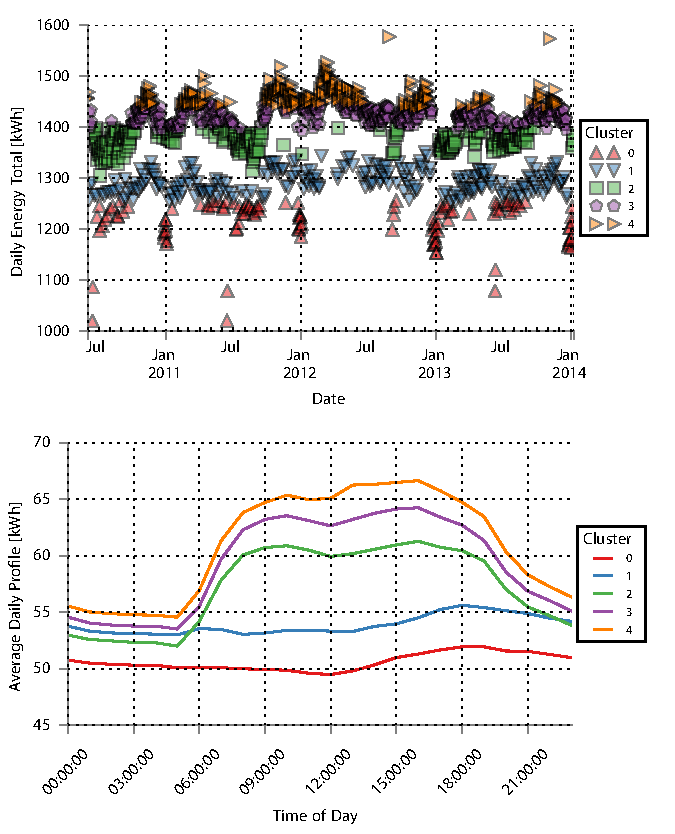
\includegraphics[height=4in]{./Data/combinedcluster}
\caption{Load profiles clusters from a building electricity consumption data set (adapted from \cite{miller_forensically_2015})}
\label{fig:clusteringexample}
\end{figure}

\subsection{Novelty Detection}
Novelty detection is a category of techniques that finds behavior or observations within a data set that are unique and often do not conform to expected behavior \cite{chandola_anomaly_2009}. Concepts such as outlier and anomaly detection fit within this category. An example of an outliers detection process can be seen in Figure \ref{fig:outlierdetectionexample} in which a set of \emph{quality analysis metrics} were implemented on a single data stream including an outliers detection component that is designated as quality level 2. Certain types of novelty detection techniques in this review include Principal Component Analysis (PCA), Generalized Additive Models (GAM), Classification and Regression Trees (CART), Wavelets, Fourier Transforms, Linear Discriminant Analysis (LDA), and Nearest Neighbor methods.

\begin{figure}[H]
\centering
\includegraphics[height=2in]{./Data/availability_singleplot}
\caption{Example of novelty detection through data quality metrics in which a value of 2 signifies and statistical outlier (adapted from \cite{miller_forensically_2015})}
\label{fig:outlierdetectionexample}
\end{figure}

\subsection{Motif and Discord Detection}
Motif and discord detection is a sub-domain unique to the investigation of time-series data sets \cite{senin_grammarviz_2014}. A motif is a subsequence of data that exhibits a pattern that frequently occurs in a data stream. A discord is a subsequence that occurs rarely and is considered anomalous amongst the rest of the data set. Figure \ref{fig:motifdiscordexample} illustrates the concept of motif and discord candidate identification on a two-week sample data set. This example is of thirteen days of electrical consumption where the diurnal patterns were extracted using Symbolic Aggregate Approximation (SAX) and divided into motif and discord candidates according to their frequency amongst the sample set. Other approaches found in the literature related to motif and discord detection include Markov Models, Maximum Likelihood, Dirichlet Process Gaussian Mixture Models (DPGMM), and Incremental Summarization and Pattern Characterization (ISPC).

\begin{figure}[ht!]
\centering
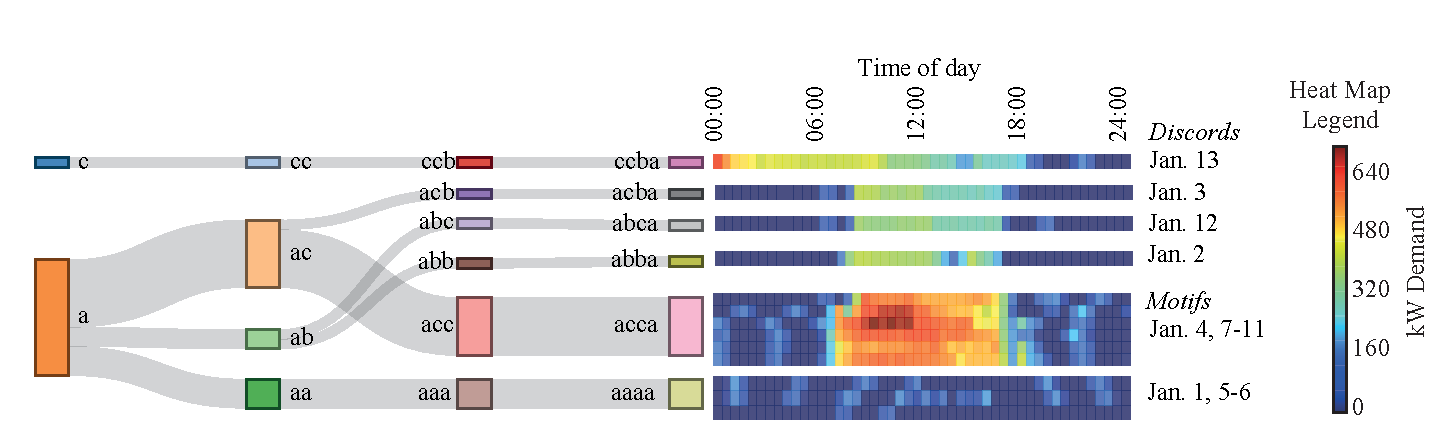
\includegraphics[height=2in]{./Data/DiscordSankeyExampleWithHeatmapV2}
\caption{Example of motif and discord candidate extraction from a two week example data set (adapted from \cite{miller_automated_2015})}
\label{fig:motifdiscordexample}
\end{figure}

\subsection{Rule Extraction}
Rule extraction techniques focus on the ability automatically to find relationships between variables within a data set. Hastie et al. describe the goal of these processes as attempting to find shared values of the variables $X = (X_1,X_2,...,X_p)$ that appear most frequently in the database \cite{hastie_elements_2009}. These rules are often used to support control sequences and fault detection approaches at the component level. The general field of creating Data Association Rules (DAC) is the most common form of this technique. Other methods found in this review include Markov Models and Support Vector Machines (SVM).

\subsection{Visual Analytics}
The domain of visual analytics is relatively new and rapidly developing. Keim et al. define the field as a medium of a semi-automated analytical process, where humans and machines cooperate using their respective distinct capabilities for the most useful results \cite{keim_visual_2008}. This domain focuses on the use of visualization and various human interactions such as the Schneiderman mantra of Overview First, Filter and Zoom, and Details-on-Demand \cite{shneiderman_eyes_1996}. Visual analytics is developing in the building industry through the proliferation of energy management system dashboards. This review divides the visual analytics for building energy into two categories: approaches focused on finding patterns in energy data and those on more general energy management with focuses on performance indicators.\\

Many of the publications in this review indicate a dominant technique that is determined and included in Sections \ref{SmartMeter}-\ref{AnomalyDetection} and their associated tables. Some of the publications don't specify a single technique or implement numerous techniques for comparison; these publications are classified under the category of \emph{Multiple Techniques}.

\section{Methodology and Overview of Publications}
\label{Overview}
This review was started through a selection of unsupervised analytics categories outlined by authoritative sources from the machine learning community \citep{hastie_elements_2009,james_introduction_2013,duda_pattern_2012,mirkin_clustering:_2012}. The categories selected are clustering, novelty detection, motif and discord detection, and rule extraction. The field of visual analytics was added to these groups to cover the presentation layer of many of these types of techniques. An initial search of publications was then selected for inclusion through a Google Scholar search of the combination of the method categories and the terms ``building energy'', ``building performance analysis'', and ``building energy analysis''. From this initial list of publications, a set of application categories and sub-categories was developed as seen in Figure \ref{fig:categoriespie}. A more detailed search of each application class was then completed to account for the unique analytics techniques used in those domains. Only publications with a majority of the focus on utilization of unsupervised techniques and with a focus only on non-residential buildings are reviewed. Only works completed since 2005 are included to discuss only the most contemporary work and due to the relatively recent development of most of the techniques examined. A cutoff date of April 1, 2016, is applied for inclusions of publications in this review.

\begin{figure}[H]
\centering
\includegraphics[height=3.5in]{./Data/PieChart_resized}
\caption{Categories and sub-categories (including number of publications) of building performance analysis applications of unsupervised learning and visual analytics}
\label{fig:categoriespie}
\end{figure}

Analysis of the publications discussed in this paper at a high level reveals insights regarding the frequency and types of techniques used, the number of publications and trend over time, and the popularity of specific publications within the domain.

\subsection{Specific Techniques}
Figure \ref{fig:techbreakdown} illustrates the frequency of use of various unsupervised and visual analytics methods in the publications reviewed. The largest specific category is papers that use numerous techniques in conjunction to achieve a complex goal. Amongst the papers that have a dominant method, K-Means clustering, data association rules, and visual analytics-based pattern analysis and energy information systems round out the top five. 

\begin{figure}[H]
\centering
\includegraphics[height=4in]{./Data/Techniques}
\caption{Breakdown of specific and general analytics techniques utilized}
\label{fig:techbreakdown}
\end{figure}

\subsection{Research Sectors}
Figure \ref{fig:yearbreakdown} illustrates the breakdown of publications based on the year published since 2005. They are further divided into four broad research domains: building energy analysis, building simulation, computer science and electrical engineering. These research field categories were subjectively determined for each paper through evaluating a combination of which university department the authors were from and in which publication the study was published. Building energy analysis pertains to researchers who predominantly focus on measured data analysis from buildings while simulation experts research forward modeling and simulation of building and urban systems. Both fields of study most often exist within architecture or mechanical engineering departments. Electrical engineering and computer science are two well-established domains and exist in their own departments. It is noticed that there is a gradual increase in the number of publications over the last ten years with electrical engineering and building energy analysis being the most common in the first few years and computer science and building simulation picking up since 2008.  

\begin{figure}[H]
\centering
\includegraphics[height=3in]{./Data/PublicationYear}
\caption{Breakdown of publications by year published and research domain}
\label{fig:yearbreakdown}
\end{figure}

\subsection{Publications Venues}
This section analyzes the prevalence of certain publication venues within this review. Figure \ref{fig:journalbreakdown} illustrates the breakdown of the publication venues represented. The Energy and Buildings Journal from the building energy analysis domain dominates this list with 17 articles. Building simulation and energy analysis research domains publish most often in this journal as well as Applied Energy and Energy Efficiency. Several IEEE conferences and journals are also dominant as most of the papers from the electrical engineering domain are in these venues.

\begin{figure}[H]
\centering
\includegraphics[height=4in]{./Data/PublicationVenues}
\caption{Breakdown of publications by publication type and research domain}
\label{fig:journalbreakdown}
\end{figure}

The next sections discuss each application category and sub-category of building performance analysis in more detail including a short overview of each publication.


\section{Smart Meter Analytics}
\label{SmartMeter}
Advanced Metering Infrastructure (AMI), also known as smart meter systems, is a network of energy meters, most often focused on the electrical power measurement of a whole building. These systems are implemented and utilized by electrical utility providers. The growth of these meters has been rapid in many parts of the world. As mentioned in Section \ref{Introduction}, there are over 58 million smart meters alone installed in the United States \cite{energy_information_administration_how_2015}. Conventional metering infrastructure only facilitates monthly data collection for billing purposes, while the new AMI framework allows for sub-hourly electrical demand readings. These data are primarily used for demand characterization and billing, however, many additional uses are being discovered. A wide-range of studies have been completed in recent years to focus on a range of issues related to automatically extracting information from these data using unsupervised techniques. In this section, three sub-categories of application are discussed: load profiling, account classification, and disaggregation. Table \ref{fig:smart_table} lists these publications and their general attributes.

{\footnotesize
\begin{longtabu} to \textwidth {
    % |X[3,l]|
    % X[3,l]|
    X[0.4,l]|
    X[1,l]|
    X[1,l]|
    X[1,l]|
    X[1,l]|
    X[0.5,l]|} %{llllrlllll}

% \everyrow{\hline}

\toprule
                                             Pub. Year & Sub-Application &             Sector &   Type of Analysis &         Technique &  Reference \\
\midrule
\endhead
\midrule
\multicolumn{4}{r}{{Continued on next page}} \\
\midrule
\endfoot

\bottomrule
\endlastfoot
2016 &  Customer Class. &    Building Energy &         Clustering &     K-Means &        \cite{jang_variability_2016} \\
2015 &   Load Profiling &   Computer Science &         Clustering &     K-Means &     \cite{shahzadeh_improving_2015} \\
2015 &  Customer Class. &   Computer Science &   Visual Analytics &    Patterns &               \cite{liu_smas:_2015} \\
2015 &   Load Profiling &  Elec. Engineering &         Clustering &         PCA &        \cite{pan_kernel-based_2015} \\
2015 &   Load Profiling &  Elec. Engineering &         Clustering &    Multiple &  \cite{panapakidis_evaluation_2015} \\
2015 &  Customer Class. &   Computer Science &  Novelty Detection &      Markov &         \cite{fagiani_novelty_2015} \\
2014 &   Disaggregation &  Elec. Engineering &    Motif Detection &         SAX &     \cite{reinhardt_powersax:_2014} \\
2014 &   Load Profiling &    Building Energy &         Clustering &     K-Means &        \cite{lavin_clustering_2014} \\
2014 &   Load Profiling &  Elec. Engineering &         Clustering &     K-Means &            \cite{green_divide_2014} \\
2014 &   Load Profiling &   Computer Science &   Visual Analytics &    Patterns &   \cite{jarrah_nezhad_smartd:_2014} \\
2014 &  Customer Class. &  Elec. Engineering &   Visual Analytics &    Multiple &              \cite{cakmak_new_2014} \\
2013 &   Disaggregation &   Computer Science &    Motif Detection &       DPGMM &           \cite{shao_temporal_2013} \\
2013 &   Load Profiling &  Elec. Engineering &         Clustering &  Ant Colony &       \cite{chicco_electrical_2013} \\
2013 &  Customer Class. &    Building Energy &         Clustering &    Multiple &        \cite{borgeson_targeted_2013} \\
2013 &   Load Profiling &  Elec. Engineering &         Clustering &    Multiple &       \cite{iglesias_analysis_2013} \\
2012 &   Load Profiling &  Elec. Engineering &         Clustering &    Multiple &            \cite{ramos_typical_2012} \\
2012 &  Customer Class. &      Building Sim. &         Clustering &    Bayesian &  \cite{florita_classification_2012} \\
2011 &   Load Profiling &  Elec. Engineering &    Motif Detection &        ISPC &           \cite{de_silva_data_2011} \\
2010 &  Customer Class. &  Elec. Engineering &         Clustering &    Multiple &       \cite{bidoki_evaluating_2010} \\
2009 &   Load Profiling &   Computer Science &         Clustering &    Multiple &       \cite{gullo_low-voltage_2009} \\
2009 &   Load Profiling &  Elec. Engineering &         Clustering &    Multiple &   \cite{rasanen_feature-based_2009} \\
2009 &   Load Profiling &  Elec. Engineering &         Clustering &         SVM &          \cite{chicco_support_2009} \\
2009 &  Customer Class. &  Elec. Engineering &         Clustering &    Multiple &                \cite{vale_data_2009} \\
2008 &  Customer Class. &   Computer Science &         Clustering &         SOM &        \cite{rasanen_reducing_2008} \\
2006 &  Customer Class. &  Elec. Engineering &         Clustering &         SOM &    \cite{verdu_classification_2006} \\
2005 &  Customer Class. &  Elec. Engineering &         Clustering &     K-Means &     \cite{figueiredo_electric_2005} \\
\\
\caption{Publications from the Smart Meter category}
\label{fig:smart_table}
\end{longtabu}
}

\subsection{Load Profiling}
Load profiling is the process of grouping temporal subsequences of measured energy data for the purpose of characterizing the typical behavior of an individual customer. It involves time-series clustering and feature extraction. Chicco et al. provide an original example in our review of this process using support vector machine clustering \cite{chicco_support_2009}. Gullo et al. and R\"as\"anen et al. took the process further by introducing a framework of various clustering procedures that were implemented on case studies \cite{gullo_low-voltage_2009,rasanen_feature-based_2009}. Ramos et al., Iglesias et al., and Panapakidis et al. tested various conventional and new clustering methods and similarity metrics to determine those most applicable to electrical load profiling \cite{iglesias_analysis_2013,ramos_typical_2012,panapakidis_evaluation_2015}. Chicco et al. explored new clustering techniques based on ant colony grouping while Pan et al. discovered the use of kernel PCA for the same purpose \cite{chicco_electrical_2013,pan_kernel-based_2015}. Several groups of researchers such as Lavin and Klabjan and Green et al. have found efficient use in using the core K-Means clustering algorithm for load profiling \cite{lavin_clustering_2014,green_divide_2014}. Shahzadeh et al. discussed the use of profiling as applied to forecast accuracy of temporal data \cite{shahzadeh_improving_2015}. Two studies diverge from the standard profile development using clustering paradigm. The first is by De Silva et al. who uses Incremental Summarization and Pattern Characterization (ISPC) instead of clustering to find load profiles \cite{de_silva_data_2011}. The other is the visual analytics-based approach of creating a smart meter analytics dashboard by Nezhad et al. to set up and inspect typical load profiles \cite{jarrah_nezhad_smartd:_2014}.

\subsection{Customer Classification}
Automated account classification is the next sub-category that utilizes unsupervised learning techniques within the smart meter domain. These methods often employ load profile clustering as a first step but differentiate themselves in using those features to classify accounts, or buildings, that fit within various categories. Therefore, account classification is a type of manual semi-supervised analysis utilizing load profiling as a basis. The study by Figueiredo et al. harnessed K-Means and a labeled sample from accounts in Portugal to showcase this concept \cite{figueiredo_electric_2005}. Verdu et al. and R\"as\"anen et al. applied self-organizing maps (SOM) to accomplish a similar study that classifies accounts according to the applicability of several demand response scenarios \cite{verdu_classification_2006,rasanen_reducing_2008}. Vale et al. give an overview of a general data mining framework focused on characterizing customers \cite{vale_data_2009}. Florita et al. diverge from the use of measured data by creating a massive amount of simulation data of load profiles to quantify energy storage applications for the power grid \cite{florita_classification_2012}. Fagiani et al. use Markov Model novelty detection to automatically classify customers who potentially have leakage or waste issues \cite{fagiani_novelty_2015}. Cakmak et al. and Liu et al. test new visual analytics techniques within more holistic analysis framework for analyzing customers \cite{cakmak_new_2014,liu_smas:_2015}. Borgeson used various clustering and occupancy detection techniques to analyze a large AMI data set from California \cite{borgeson_targeted_2013}. Bidoki et al. tested various clustering techniques to evaluate applicability for customer classification \cite{bidoki_evaluating_2010}. A recent study in Korea develops a new clustering method for segmenting customers to analyze demand response incentives \cite{jang_variability_2016}.

\subsection{Disaggregation}
The last area of smart meter data analysis is the field of meter disaggregation. Disaggregation attempts decompose a measurement signal from a high level reading to the individual loads being measured. This domain is well-researched from a supervised model perspective but recent attempts at unsupervised, pattern-based disaggregation were developed to facilitate implementation on unlabeled smart meter data. Shao et al. use Dirichlet Process Gaussian Mixture Models to find and disaggregate patterns in sub-hourly meter data \cite{shao_temporal_2013}. Reinhardt and Koessler use a version of symbolic aggregate approximation (SAX) to extract and identify disaggregated patterns for the purpose of prediction \cite{reinhardt_powersax:_2014}. These studies are also unique in that few of the disaggregation studies focus on commercial buildings as opposed to residential buildings.

\section{Portfolio Analytics}
\label{PortfolioAnalytics}

Portfolio analysis is a domain in which a large group of buildings, often located in the same geographical area or owned or managed by the same entity, are analyzed for the purpose of managing or optimizing the group as a whole. Each subsection covers the publications reviewed in this domain that fall into three categories: characterization, classification, and targeting. Table \ref{fig:portfolio_table} illustrates an overview of all the publications in this section in addition to their attributes. 

{\footnotesize
\begin{longtabu} to \textwidth {
    % |X[3,l]|
    % X[3,l]|
    X[0.3,l]|
    X[1.3,l]|
    X[1,l]|
    X[1,l]|
    X[0.7,l]|
    X[0.5,l]|} %{llllrlllll}

% \everyrow{\hline}

\toprule
Pub. Year & Sub-Application &             Sector &   Type of Analysis &         Technique &  Reference \\
\midrule
\endhead
\midrule
\multicolumn{4}{r}{{Continued on next page}} \\
\midrule
\endfoot

\bottomrule
\endlastfoot
2016 &         Targeting &    Building Energy &         Clustering &  Fuzzy Clust. &       \cite{schlueter_analysis_2016} \\
2016 &         Targeting &    Building Energy &         Clustering &      Multiple &        \cite{geyer_application_2016} \\
2015 &  Characterization &      Building Sim. &         Clustering &      Multiple &      \cite{miller_forensically_2015} \\
2015 &  Characterization &    Building Energy &   Visual Analytics &           EIS &    \cite{yarbrough_visualizing_2015} \\
2015 &  Characterization &    Building Energy &    Motif Detection &           SAX &         \cite{miller_automated_2015} \\
2015 &  Characterization &  Elec. Engineering &   Visual Analytics &           EIS &       \cite{diong_establishing_2015} \\
2015 &       Classifying &    Building Energy &         Clustering &      Multiple &        \cite{pieri_identifying_2015} \\
2014 &       Classifying &  Elec. Engineering &  Novelty Detection &           GAM &  \cite{ploennigs_e2-diagnoser:_2014} \\
2014 &  Characterization &      Building Sim. &   Visual Analytics &      Patterns &     \cite{georgescu_site-level_2014} \\
2014 &       Classifying &    Building Energy &         Clustering &       K-Means &     \cite{heidarinejad_cluster_2014} \\
2013 &  Characterization &   Computer Science &   Visual Analytics &      Patterns &           \cite{moran_analysis_2013} \\
2013 &         Targeting &    Building Energy &    Rule Extraction &           DAR &             \cite{cabrera_data_2013} \\
2012 &       Classifying &  Elec. Engineering &         Clustering &      Multiple &     \cite{nikolaou_application_2012} \\
2012 &         Targeting &    Building Energy &         Clustering &            ML &     \cite{petcharat_assessment_2012} \\
2012 &  Characterization &      Building Sim. &         Clustering &       K-Means &            \cite{an_estimation_2012} \\
2011 &         Targeting &   Computer Science &  Novelty Detection &        Markov &          \cite{bellala_towards_2011} \\
2011 &  Characterization &    Building Energy &   Visual Analytics &           EIS &        \cite{lehrer_visualizing_2011} \\
2010 &  Characterization &    Building Energy &   Visual Analytics &           EIS &      \cite{granderson_building_2010} \\
2010 &         Targeting &    Building Energy &         Clustering &      Multiple &            \cite{gaitani_using_2010} \\
2009 &         Targeting &   Computer Science &         Clustering &            ML &         \cite{sedano_improving_2009} \\
2009 &  Characterization &    Building Energy &   Visual Analytics &           EIS &          \cite{lehrer_research_2009} \\
2009 &  Characterization &   Computer Science &   Visual Analytics &           EIS &           \cite{agarwal_energy_2009} \\
2008 &  Characterization &    Building Energy &  Novelty Detection &           PCA &            \cite{lam_principal_2008} \\
2007 &       Classifying &    Building Energy &         Clustering &  Fuzzy Clust. &        \cite{santamouris_using_2007} \\
2005 &  Characterization &    Building Energy &         Clustering &  Hierarchical &             \cite{seem_pattern_2005} \\
\\
\caption{Publications from the Portfolio Analysis category}
\label{fig:portfolio_table}
\end{longtabu}
}

\subsection{Characterization}
Publications that address the characterization of a portfolio of buildings include unsupervised techniques meant to evaluate and visualize the range of behaviors and performance of the group. A majority of the techniques utilized are either clustering or visual analytics that provide a model of exploratory analysis that enable further steps. Seem produced an influential study that extracts days of the week with similar consumption profiles \cite{seem_pattern_2005}. Further clustering work was completed by An et al. to estimate thermal parameters of a portfolio of buildings \cite{an_estimation_2012}. Lam et al. used Principal Component Analysis to extract information about a group of office buildings \cite{lam_principal_2008}. Approaches focused on visual analytics and dashboards were completed by Agarwal et al., Lehrer, and Lehrer and Vasudev \cite{agarwal_energy_2009,lehrer_research_2009,lehrer_visualizing_2011}. Granderson et al. completed a case study-based evaluation of energy information systems, in which some methods combine some unsupervised approaches with visualization \cite{granderson_building_2010}. Diong et al. completed a case study as well focused on a specific energy information system implementation  \cite{diong_establishing_2015}. Mor\'an et al. and Georgescu and Mezic developed hybrid methods that employed visual continuous maps and Koopman Operator methods respectively to visualize portfolio consumption\cite{moran_analysis_2013,georgescu_site-level_2014}. Miller et al. completed two studies focused on the use of screening techniques to automatically extract diurnal patterns from performance data and use those patterns to characterize the consumption of a portfolio of buildings  \cite{miller_forensically_2015,miller_automated_2015}. Yarbrogh et al. used visual analytics techniques to analyze peak demand on a university campus \cite{yarbrough_visualizing_2015}.

\subsection{Classification}
The concept of classifying buildings within a portfolio supplements the characterization techniques by assigning individual buildings to subgroups of relative performance for the purpose of benchmarking or decision-making. Santamouris et al. produced a report using clustering and classification to assign schools in Greece to subgroups of similar performance \cite{santamouris_using_2007}. Nikolaou et al. and Pieri et al. further extended this type of work to office buildings and hotels\cite{nikolaou_application_2012,pieri_identifying_2015}. Heidarinejad et al. released an analysis of clustered simulation data to classify LEED-certified office buildings \cite{heidarinejad_cluster_2014}. Ploennigs et al. created a platform for monitoring, diagnosing and classifying buildings and operational behavior within a portfolio to quickly visualizing the outputs \cite{ploennigs_e2-diagnoser:_2014}.

\subsection{Targeting}
Targeting is a concept that builds upon characterization and classification to identify specific buildings or measures to be implemented in a portfolio to improve performance. These publications are differentiated in that specific measures are identified in the analysis. Sedano et al. use Cooperative Maximum-Likelihood amongst other techniques to evaluate the thermal insulation performance of buildings \cite{sedano_improving_2009}. Gaitani et al. used PCA and clustering to target heating efficiency in school buildings \cite{gaitani_using_2010}. Bellala et al. used various methods to find lighting energy savings on a campus of a large organization \cite{bellala_towards_2011}. Petcharat et al. also found lighting energy savings in a group of buildings \cite{petcharat_assessment_2012}. Cabrera and Zareipour used data association rules to complete a similar study to find wasteful patterns \cite{cabrera_data_2013}. Geyer et al.  and Schlueter et al. test various clustering strategies to group different buildings within a Swiss alpine village according to their applicability for retrofit interventions \cite{geyer_application_2016} and thermal micro-grid feasibility \cite{schlueter_analysis_2016}.

\section{Operations, Optimization, and Controls}
\label{Operations}
Unsupervised techniques focused on individual buildings themselves are placed in the category for building operations, optimization, and control. This class contains the largest number of publications, and it incorporates a wider range of applications. It is differentiated from Section \ref{AnomalyDetection} in that the applications are not as focused on detecting and fixing the anomalous behavior. This section evaluates publications within the sub-categories of occupancy detection, retrofit analysis, controls, and energy management. Table \ref{fig:operations_table} outlines the publications in this section and their key attributes.

{\footnotesize
\begin{longtabu} to \textwidth {
    % |X[3,l]|
    % X[3,l]|
    X[0.3,l]|
    X[1.3,l]|
    X[1,l]|
    X[1,l]|
    X[0.7,l]|
    X[0.5,l]|} %{llllrlllll}

% \everyrow{\hline}

\toprule
Pub. Year & Sub-Application &             Sector &   Type of Analysis &         Technique &  Reference \\
\midrule
\endhead
\midrule
\multicolumn{4}{r}{{Continued on next page}} \\
\midrule
\endfoot

\bottomrule
\endlastfoot
2016 &  Occupancy Detection &    Building Energy &   Rule Extraction &  Wavelets &                 \cite{ahn_correlation_2016} \\
2015 &  Occupancy Detection &   Computer Science &        Clustering &   K-Means &                 \cite{mansur_learning_2015} \\
2015 &  Occupancy Detection &    Building Energy &   Rule Extraction &    Markov &       \cite{adamopoulou_context-aware_2015} \\
2015 &    Energy Management &    Building Energy &   Rule Extraction &       DAR &                    \cite{fan_temporal_2015} \\
2015 &    Energy Management &    Building Energy &  Visual Analytics &       EIS &                      \cite{gayeski_data_2015} \\
2015 &  Occupancy Detection &    Building Energy &   Rule Extraction &  Multiple &                  \cite{doca_occupancy_2015} \\
2015 &             Controls &  Elec. Engineering &   Motif Detection &       SAX &                   \cite{habib_finding_2015} \\
2014 &    Energy Management &    Building Energy &   Rule Extraction &       DAR &                       \cite{xiao_data_2014} \\
2014 &             Controls &  Elec. Engineering &   Rule Extraction &       SVM &               \cite{domahidi_learning_2014} \\
2013 &    Energy Management &  Elec. Engineering &  Visual Analytics &  Patterns &               \cite{lange_discovering_2013} \\
2013 &             Controls &    Building Energy &        Clustering &  Multiple &                \cite{bogen_evaluating_2013} \\
2013 &    Energy Management &      Building Sim. &   Rule Extraction &       DAR &                     \cite{yu_extracting_2013} \\
2013 &             Controls &      Building Sim. &   Rule Extraction &       DAR &        \cite{may-ostendorp_extraction_2013} \\
2013 &             Controls &    Building Energy &        Clustering &   K-Means &                  \cite{fan_prediction_2013} \\
2013 &             Controls &   Computer Science &        Clustering &       EMC &                    \cite{hong_towards_2013} \\
2012 &    Energy Management &  Elec. Engineering &  Visual Analytics &  Patterns &                    \cite{lange_energy_2012} \\
2012 &  Occupancy Detection &  Elec. Engineering &   Motif Detection &        ML &        \cite{thanayankizil_softgreen:_2012} \\
2011 &             Controls &    Building Energy &   Rule Extraction &       DAR &  \cite{may-ostendorp_model-predictive_2011} \\
2011 &    Energy Management &    Building Energy &  Visual Analytics &       EIS &             \cite{duarte_prioritizing_2011} \\
2011 &  Occupancy Detection &   Computer Science &        Clustering &  Multiple &                  \cite{augello_sensor_2011} \\
2011 &  Occupancy Detection &      Building Sim. &   Motif Detection &    Markov &                   \cite{dong_building_2011} \\
2011 &             Controls &   Computer Science &  Visual Analytics &  Patterns &                 \cite{hao_visualizing_2011} \\
2010 &             Controls &   Computer Science &   Motif Detection &       SAX &                    \cite{patnaik_data_2010} \\
2009 &             Controls &   Computer Science &   Motif Detection &       SAX &             \cite{patnaik_sustainable_2009} \\
2008 &             Controls &  Elec. Engineering &        Clustering &  Multiple &         \cite{kusiak_clustering-based_2008} \\
\\
\caption{Publications from the Operations, Optimization, and Controls category}
\label{fig:operations_table}
\end{longtabu}
}

\subsection{Occupancy Detection}
Occupancy detection using unsupervised techniques infers human presence in a non-residential building without a labeled ground truth dataset or as part of a semi-supervised approach using a subset of labeled data. This occupancy detection is then used for analysis or as inputs for control of systems. Augello et al. used multiple techniques to infer occupant presence on a campus in Italy \cite{augello_sensor_2011}. Dong and Lam  used Hidden Markov Models to detect occupancy patterns that were then used in a simulation \cite{dong_building_2011}. Thanayankizil et al. developed a concept called Context Profiling in which occupancy was detected temporally and spatially \cite{thanayankizil_softgreen:_2012}. Mansur et al. used clustering to detect occupancy patterns from sensor data \cite{mansur_learning_2015}. The newest studies by Adamopoulou et al. and D'Oca and Hong use a range of techniques to extract rules related to occupancy \cite{adamopoulou_context-aware_2015,doca_occupancy_2015}. A recent study using wavelets illustrates the correlation of occupancy with actual energy consumption \cite{ahn_correlation_2016}.

\subsection{Controls}
Controls optimization is an enduring field of study aimed at creating a state of the best operation and energy performance for a building system such as heating, cooling, ventilation or lighting. Kusiak and Song created a means of optimally controlling a heating plant with clustering as a key step \cite{kusiak_clustering-based_2008}. Patnaik et al. completed studies focused on using motif detection to find modes of chilled water plant operation that proved most optimal \cite{patnaik_data_2010,patnaik_sustainable_2009}. Hao et al. built upon these concepts to create a visual analytics tool to investigate these motifs \cite{hao_visualizing_2011}. May-Ostendorp et al. used rule extraction as a means of enhancing a model-predictive control process of mixed-mode systems \cite{may-ostendorp_model-predictive_2011,may-ostendorp_extraction_2013}. Bogen et al. used clustering to detect usage patterns for building control system evaluation \cite{bogen_evaluating_2013}. Fan et al. used clustering to enhance chiller power prediction with the ultimate goal of control optimization \cite{fan_prediction_2013}. Hong et al. used Empirical Mode Decomposition to spatially optimize the placement of sensors in a building \cite{hong_towards_2013}. Domahidi et al. used support vector machines (SVM) to extract optimized rules for supervisory control \cite{domahidi_learning_2014}. Habib and Zucker use SAX to identify common motifs of an absorption chiller for the purpose of characterization and control \cite{habib_finding_2015}.

\subsection{Energy Management}
Energy management and analysis of an individual building using unsupervised techniques is becoming common due to the increasing amounts of raw building management (BMS) and energy management system (EMS) data. Users of these techniques are often facilities management professionals or consultants who undertake the process to understand how the building is consuming energy. Duarte et al. use visual analytics to process data from an EMS along with various pre-processing techniques \cite{duarte_prioritizing_2011}. Lange et al. created two overview studies focused spatiotemporal visualization of building performance data and its interpretation in various case studies \cite{lange_energy_2012,lange_discovering_2013}. Gayeski et al. completed a recent survey of operations professionals on their use of graphical interfaces of BMS and EMS dashboards \cite{gayeski_data_2015}. Outside of the visual analytics realm, Fan et al., Xiao and Fan, and Yu et al. completed studies of an entire data mining using framework using data association rules to improve operational performance \cite{fan_temporal_2015,xiao_data_2014,yu_extracting_2013}.

\section{Anomaly Detection}
\label{AnomalyDetection}
Anomaly detection for buildings focuses on the detection and diagnostics of problems occurring within a building, its subsystems, and components. This field is most often focuses on the use of novelty detection or clustering approaches to find anomalous behavior. The sub-categories for this section are divided according to the spatial hierarchy of systems within a building; the highest level is whole building consumption, down to the subsystems such as heating, cooling or lighting and then to the individual components of those systems. Table \ref{fig:anom_table} provides an overview of the publications in this category.

{\footnotesize
\begin{longtabu} to \textwidth {
    % |X[3,l]|
    % X[3,l]|
    X[0.4,l]|
    X[1,l]|
    X[1,l]|
    X[1,l]|
    X[1,l]|
    X[0.5,l]|} %{llllrlllll}

% \everyrow{\hline}

\toprule
Pub. Year & Sub-Application &             Sector &   Type of Analysis &         Technique &  Reference \\
\midrule
\endhead
\midrule
\multicolumn{4}{r}{{Continued on next page}} \\
\midrule
\endfoot

\bottomrule
\endlastfoot
2015 &  Whole Building &    Building Energy &  Novelty Detection &               DAR &           \cite{fan_framework_2015} \\
2015 &  Whole Building &    Building Energy &  Novelty Detection &          Multiple &         \cite{capozzoli_fault_2015} \\
2015 &       Subsystem &  Elec. Engineering &  Novelty Detection &               DAR &           \cite{sun_efficient_2015} \\
2014 &       Subsystem &    Building Energy &  Novelty Detection &               PCA &          \cite{li_model-based_2014} \\
2014 &  Whole Building &  Elec. Engineering &  Novelty Detection &               GAM &        \cite{chen_statistical_2014} \\
2014 &  Whole Building &    Building Energy &         Clustering &           K-Means &          \cite{chou_real-time_2014} \\
2014 &       Subsystem &   Computer Science &  Novelty Detection &          Multiple &     \cite{wijayasekara_mining_2014} \\
2014 &       Subsystem &      Building Sim. &  Novelty Detection &               PCA &      \cite{le_cam_application_2014} \\
2013 &  Whole Building &  Elec. Engineering &  Novelty Detection &               GAM &    \cite{ploennigs_exploiting_2013} \\
2013 &  Whole Building &   Computer Science &   Visual Analytics &          Patterns &        \cite{janetzko_anomaly_2013} \\
2013 &       Component &   Computer Science &  Novelty Detection &               EMC &         \cite{fontugne_mining_2013} \\
2013 &  Whole Building &   Computer Science &  Novelty Detection &          Multiple &          \cite{fontugne_strip_2013} \\
2012 &       Subsystem &  Elec. Engineering &  Novelty Detection &  Nearest Neighbor &     \cite{linda_computational_2012} \\
2012 &       Component &    Building Energy &  Novelty Detection &          Wavelets &               \cite{zhu_fault_2012} \\
2012 &  Whole Building &  Elec. Engineering &  Novelty Detection &           Fourier &          \cite{wrinch_anomaly_2012} \\
2012 &       Component &    Building Energy &    Rule Extraction &               DAR &                \cite{yu_novel_2012} \\
2010 &  Whole Building &   Computer Science &  Novelty Detection &              CART &              \cite{liu_method_2010} \\
2010 &  Whole Building &      Building Sim. &         Clustering &      Hierarchical &         \cite{jacob_black-box_2010} \\
2010 &       Subsystem &    Building Energy &  Novelty Detection &               PCA &       \cite{wang_system-level_2010} \\
2010 &       Subsystem &   Computer Science &   Visual Analytics &          Patterns &        \cite{forlines_wakame:_2010} \\
2008 &       Subsystem &  Elec. Engineering &  Novelty Detection &               LDA &  \cite{yoshida_identification_2008} \\
2006 &  Whole Building &    Building Energy &  Novelty Detection &              GESD &              \cite{seem_using_2006} \\
2005 &       Component &    Building Energy &  Novelty Detection &               PCA &       \cite{wang_sensor-fault_2005} \\
\\
\caption{Publications from the Anomaly Detection category}
\label{fig:anom_table}
\end{longtabu}
}

\subsection{Whole Building}
Whole building anomaly detection uses the electricity or heating and cooling energy supply in coming to a building to determine sub-sequences of poor performance. This category is complimentary to many of the Smart Meter solutions as they both focus on the use of a single data stream for a building. Seem had an early work again in this category with his work in using novelty detection to find abnormal days of consumption in buildings \cite{seem_using_2006}. Liu et al. used classification and regression trees (CART) \cite{liu_method_2010} and Wrinch et al. use frequency domain analysis for the same purpose \cite{wrinch_anomaly_2012}. Jacob et al. utilized hierarchical clustering to use as variables in regression models for whole building monitoring \cite{jacob_black-box_2010}. Fontugne et al. created a process known as the \emph{Strip, Bind, and Search} method to automatically uncover misbehavior from the whole building level and subsequently detects the source of the anomaly \cite{fontugne_strip_2013}. Janetzko et al. developed a visual analytics platform to highlight anomalous behavior in power meter data \cite{janetzko_anomaly_2013}. Chou and Telaga created a hybrid whole building anomaly detection process using K-means \cite{chou_real-time_2014}. Ploennigs et al. and Chen et al. created similar systems that use generalized additive models (GAM) \cite{ploennigs_exploiting_2013,chen_statistical_2014}. In the most recent work, Capozzoli et al. and Fan et al. use various techniques as part of a framework to detect and diagnose performance problems \cite{capozzoli_fault_2015,fan_framework_2015}. 

\subsection{Subsystems}
Subsystem anomaly detection focuses on the use of a broader data set to detect and diagnose faults from a lower level. Yoshida et al. provided a semi-supervised approach that seeks to determine which variables within a building are most influential in contributing to overall building performance  \cite{yoshida_identification_2008}. Wang et al. use PCA to diagnose sensor failures \cite{wang_system-level_2010}. Forlines and Wittenberg visualized multi-dimensional data using what they call the Wakame diagram \cite{forlines_wakame:_2010}. Linda et al. and Wijayasekara et al. use various techniques to diagnose system faults and visualize them spatially \cite{linda_computational_2012,wijayasekara_mining_2014}. Le Cam et al. use PCA to create inverse models to detect problems in HVAC systems \cite{le_cam_application_2014}. Li and Wen created a similar process using PCA in conjunction with wavelet transform \cite{li_model-based_2014}. Sun et al. used data association rules to create fault detection thresholds for finding anomalies \cite{sun_efficient_2015}.

\subsection{Components}
Component level anomaly detection is a bottom-up fault detection approach that focuses on determining faults in individual equipment. Wang and Cui use PCA to detect component faults in chilled water plants  \cite{wang_sensor-fault_2005}. Yu et al. and Fontugne et al. both compliment their work at the whole building level to find associated component performance anomalies automatically \cite{yu_novel_2012,fontugne_mining_2013}. Zhu et al. use wavelets to diagnose issues in air handling units (AHU) \cite{zhu_fault_2012}.


\section{Discussion}
\label{discussion}

\subsection{Challenges}
Several challenges facing the use of unsupervised machine learning in building performance were uncovered through this process of review. The first relates to the effect of several traditional research sectors exploring techniques targeted on the improvement of building performance. It was found that different sets of terminology are used to describe similar concepts. For example, in the building energy analysis field, the term \emph{fault} (such as \cite{zhu_fault_2012}) is used to describe a situation that is similar to what is labeled an \emph{anomaly} in the data mining domain (such as \cite{fontugne_mining_2013}). Thus, discussions between these fields are restrained and completing a review of knowledge is difficult.

Another critical issue related to differences in domains is the inconsistency of success objectives. Often individual papers would discuss the accuracy or efficiency of the algorithm or technical process itself (such as \cite{iglesias_analysis_2013}), while others focused exclusively on the end results of the evaluation such as how much energy was saved (such as \cite{seem_using_2006}). Several examples publications successfully address both types of issues. For example, Ploennings et al. published studies which both addressed the applicability of generalized additive models and discussed their implementation in a platform that is applied to real buildings \cite{ploennigs_exploiting_2013,ploennigs_e2-diagnoser:_2014}. Researchers should strive to optimize in both the theoretical and practical domains to have the most impact on real buildings.

Another observation relates to the lack of easy reproducibility amongst studies. Reproducibility provides the ability for a third-party researcher to easily recreate the results of a study through a release of the data or code developed. Recent prominent articles have outlined the importance of reproducibility in science \cite{_journals_2014} and the sharing of data and code to enhance this pursuit \cite{_code_2014}. The biomedical sciences research community is leading the way in this effort; editors from over 30 major journals, funding agency representatives, and scientific leaders from that field created guidelines for the enhancement of reproducibility \cite{_journals_2014}. Research from the building performance analysis community should follow this lead, specifically on machine learning and other types of empirical analysis.

Another challenge discovered is the lack of clarity regarding which is the optimal technique for each application. For example, a number of studies were completed to test the ability of clustering techniques to group similar daily load profiles \cite{chicco_support_2009,de_silva_data_2011,green_divide_2014,gullo_low-voltage_2009,lavin_clustering_2014,ramos_typical_2012,shahzadeh_improving_2015}. A researcher or analyst who is searching for the best technique can see a survey of implementations through these publications; however, it's hard for them to be compared against each other as each utilizes a different data set and incorporates different methodologies. An explanation of the amount of effort needed to implement a technique is missing in most studies as well. For example, in order to implement a certain algorithm on a potential use-case or data set, an analyst is interested in which parameters need to be tuned, what labeled ground truth data should be gathered, and what expertise is necessary for understanding and implementation. This lack of comparison stifles the ability to make conclusions about the efficiency, interpretability, and appropriateness of use of each algorithm. 

\subsection{Opportunities}
To address the challenges related to interdisciplinary collaboration, an opportunity exists for better dialogue between the electrical engineering, computer science, and building performance and simulation analysis research communities through cross-disciplinary venues that encourage submission of works from all domains. Several publication venues were found that publish papers written by academics from diverse backgrounds. IEEE and ACM conferences, in particular, were found to be somewhat diverse as compared to other publication outlets. The further development of these avenues will create a more welcoming environment in which different disciplines can exchange terminology, objectives, and culture.

Concerning reproducibility, the release of specific data sets for data science publications could become the norm, thus facilitating the ability for a third-party to recreate the results. The authors have published several recent papers with this situation \cite{miller_forensically_2015,miller_automated_2015}. These publications include a sample data set and a set of Jupyter notebooks that can be downloaded and used to replicate the results of those studies easily. The Jupyter notebook website states that it is "an open source, web application-based document that combines live code, equations, visualizations, and explanatory text."\footnote{https://jupyter.org/} The use of these types of formats is an opportunity to enhance the interdisciplinary communication further through the sharing and utilization of publication data.

The final opportunity relates to the ambiguity of algorithm applicability amongst a set of publications. This phenomenon is observed in the wider data mining community as a whole \cite{keogh_need_2003}. In their study, Keogh et al. describe a scenario in which ``Literally hundreds of papers have introduced new algorithms to index, classify, cluster, and segment time series.'' They go on to state, ``Much of this work has very little utility because the contribution made (speed in the case of indexing, accuracy in the case of classification and clustering, model accuracy in the case of segmentation) offer an amount of improvement that would have been completely dwarfed by the variance that would have been observed by testing on many real world datasets, or the variance that would have been observed by changing minor (unstated) implementation details.'' They make the case that time series benchmarking data sets should be used to evaluate whether a new proposed algorithm is more beneficial as compared to previous work. The use of benchmark data sets reduces the impact of implementation bias, the disparity in the quality of implementation of a proposed approach versus its competitors, and data bias, the use of a particular set of testing data to confirm a desired finding. These biases were proven common amongst popular data mining publications, and it is suspected that they may be prevalent in the papers in this review. Benchmarking data sets for building performance analysis could be developed and promoted for use in papers similar to what was used in the \emph{Great Building Energy Predictor Shootout} competition that was held in the mid-1990's \cite{kreider_predicting_1994}. In this competition, standardized training and testing data sets were provided to numerous participants to determine who could create the most accurate model to predict future consumption. A modern-day \emph{energy predictor shootout} could be held to incorporate the numerous advances made in machine learning since then. In addition to the ability to compare accuracy of algorithms, publications should also include more detailed explanations of the effort required to implement the proposed techniques such that a third-party could evaluate whether the effort-to-accuracy balance is right for their application. 

\section{Conclusion}
This review provides an overview of publications from several research domains that utilize unsupervised statistical learning and visual analytics as applied to non-residential building performance analysis. The publications are categorized according to machine learning technique and application and sub-application of utilization. Clustering algorithms, and especially the K-Means algorithm, stand out as popular amongst most of the application domains. Visual analytics approaches are also quite popular as generally applied techniques. Almost half of the procedures implemented were only observed once in the publications as a dominant approach; thus, there is an opportunity to explore their potential further. The papers selected increase in number steadily over the last decade with computer science and electrical engineering slowly identifying the non-residential building industry as an excellent target for implementation of developed techniques. The dominant publication venues in this review came from the building energy analysis domain. However, many other publication venues are quickly catching up due to the increase of \emph{big data} sources from the building and urban environments. Several key challenges were identified through this process, including a noticeable divide between several research communities, a diverse set of objectives, and the lack of reproducible studies. The need for open, benchmarking data sets is discussed and potential improvements are suggested.

\section{Acknowledgments}
This research was funded through a Fellowship from the Institute of Technology in Architecture from the ETH Zurich.



\bibliographystyle{elsarticle-num}
%\bibliographystyle{elsarticle-harv}
% \bibliographystyle{elsarticle-num-names}
% \bibliographystyle{model1a-num-names}
% \bibliographystyle{model1b-num-names}
% \bibliographystyle{model1c-num-names}
% \bibliographystyle{model1-num-names}
% \bibliographystyle{model2-names}
% \bibliographystyle{model3a-num-names}
% \bibliographystyle{model3-num-names}
% \bibliographystyle{model4-names}
% \bibliographystyle{model5-names}
% \bibliographystyle{model6-num-names}

\bibliography{unsupervisedreview}

\end{document}

%%
%% End of file `elsarticle-template-num.tex'.
